
%% Template Elsevier for Neuroimage

%% Use the option review to obtain double line spacing
%\documentclass[authoryear,preprint,review]{elsarticle}
\documentclass[authoryear]{elsarticle}
%\usepackage[framed,numbered,autolinebreaks,useliterate]{mcode}
\usepackage[framed,autolinebreaks,useliterate]{mcode}
\usepackage{natbib}
\usepackage{amsmath}
%\usepackage{lineno}
\usepackage{rotating}

\usepackage{hyperref}
\usepackage{amssymb}
\usepackage{amsfonts}


%\usepackage{algorithm2e}
%\usepackage{algorithmic}
%\usepackage{todonotes}
\usepackage{pdflscape}
\journal{Neuroimage}
\usepackage{color,transparent}
%\usepackage{color} 
%\pdfoptionpdfminorversion 6
\pdfminorversion=5

%\usepackage{graphicx}
%\usepackage{subcaption}
%\usepackage{mwe}
\usepackage{subfig}
\usepackage{caption}
%\usepackage{subcaption}
\usepackage{setspace}
\usepackage{lineno}
\linenumbers

\begin{document}

% Title must be 150 words or less
\begin{frontmatter}
%\title{Feasibility of multi-centric fMRI connectivity studies of Alzheimer's disease}
%\title{Feasibility of multi-centric fMRI connectivity and impact }

%\title{Measurement bias and statistical power in multi-centric resting-state fMRI connectivity}
\title{Statistical power and measurement bias in multisite resting-state fMRI connectivity}


%\title{A power analysis for multisite studies in resting-state functional connectivity, with an application to clinical trials in Alzheimer's disease}

\author[a,b]{Christian~Dansereau}
\author[a]{Yassine~Benhajali}
\author[c]{Celine~Risterucci}
\author[c]{Emilio~Merlo Pich}
\author[a]{Pierre~Orban}
\author[d]{Douglas~Arnold}
\author[a,b]{Pierre~Bellec\corref{cor1}}
\ead{pierre.bellec@criugm.qc.ca}
\cortext[cor1]{Corresponding author}
\address[a]{Centre de Recherche de l'Institut Universitaire de G\'eriatrie de Montr\'eal, Montr\'eal, CA}
\address[b]{D\'epartement d'Informatique et de recherche op\'erationnelle, Universit\'e de Montr\'eal, Montr\'eal,CA}
\address[c]{F. Hoffmann-La Roche Ldt., Basel, Switzerland}
\address[d]{NeuroRx, Montreal, Quebec, Canada}

% Please keep the abstract between 250 and 300 words
%\emph{I corrected some passive voice to active voice. Passive voice in the scientific literature is incredibly annoying, although it has some popularity. Just imagine a book with sentences like ``The car was driven to the store. The food was purchased and carried back to the car.''}
\begin{abstract}

\textit{Purpose:} Studies collecting brain images at multiple sites are becoming increasingly common in resting-state functional magnetic resonance imaging (rs-fMRI) an imaging modality looking at the functional brain dynamics. Some initiative have already started to share rs-fMRI data from multiple independent studies of comparable populations, with the objective of dramatically increasing the sample-size at the cost of decreased sample homogeneity. We propose to quantify the size of the difference in average connectivity (bias) introduce by the pooling of multiple sites and its impact on our capacity to detect effects in rs-functional connectivity measures.\\
\textit{Materials and Methods:} We investigated real fMRI datasets collected across eight scanning sites with 3T scanners and heterogeneous scanning protocols, drawn from the 1000 functional connectome project. We first used this sample to characterize the amplitude of site bias in connectivity measures, as well as how this bias was distributed across brain networks. We then implemented a series of Monte-Carlo simulations, based on real data, to evaluate the impact of multisite bias on detection power in statistical tests comparing two groups with a general linear model. As a reference, we also implemented the same simulations with fMRI data collected at a single site using a sample-size equivalent to all the multisite data combined.\\
\textit{Results:} The effect size of the inter-site absolute bias in connectivity was found to be of 0.33 express in Cohen's $d$. Simulations revealed that using a heterogeneous sites slightly decrease our ability to detect changes compared to a monosite study of equivalent sample-size although this difference tend to diminish as we increase the total sample-size to a point where the difference between a monosite and a multisite dataset are negligible.\\
\textit{Conclusion:} Typical functional network were reliably found in all the sites and we found that these results support the feasibility of multisite study in rs-fMRI and in particular of pooled datasets from heterogeneous nature. We also found that the size of the site-effect was deemed small-to-moderate, which suggests that the impact of additive inter-site bias on statistical tests will be limited.


\end{abstract}

%-- 
\begin{keyword}
multisite \sep multiprotocol \sep bias \sep statistical power \sep sample-size \sep resting-state \sep fMRI, connectivity
%fmri \sep effect size \sep multisite \sep clinical trial \sep AD biomarker
\end{keyword}
\end{frontmatter}

% Unique number for each line
%\linenumbers
%\listoftodos

\section*{Highlights}

\begin{itemize}
\item Quantified the systematic measurement bias in multisite studies for heterogeneous datasets. 
\item Typical networks were reliably found across sites.
\item Some site are more biased than others.
\item Quantify the spatial distribution of the site variance.
\item Site-effect decrease with sample-size to a point of marginality.
\item Debalancing sites are not more affected in multisite than monosite studies.
\item The inter-subject contribution in term of effect size was found to be of 0.33 Cohen's $d$ compared to the inter-site contribution.
\item Multivariate analysis learn to be invariant to multisite effect.
\end{itemize}

\section{Introduction}

% Magic paragraph
\paragraph{Main objective}
Multisite studies are becoming increasingly common in resting-state functional magnetic resonance imaging (rs-fMRI). In particular, some consortia have retrospectively pooled rs-fMRI data from multiple independent studies comparing clinical cohorts with control groups, e.g. normal controls in the 1000 functional connectome project (FCP) \citep{Biswal2010}, children and adolescents suffering from attention deficit hyperactivity disorder from the ADHD200 \citep{ADHD200,Fair2012}, individual diagnosed with autism spectrum disorder in ABIDE \citep{Nielsen2013}, individuals suffering from schizophrenia REFPORBAN, or elderly subjects suffering from mild cognitive impairment \citep{Tam2015}. The rationale behind such initiatives is to dramatically increase the sample-size at the cost of decreased sample homogeneity. The systematic variations of connectivity measures derived using different scanners, called site-effects, may decrease the statistical power of group comparisons, and somewhat mitigate the benefits of having a large sample-size. In this work, our main objective was to quantitatively assess the impact of site-effects on group comparison in rs-fMRI connectivity.

\paragraph{Group comparison in rs-fMRI connectivity}
We focused in this work on the most common measure of individual functional connectivity, which is the Pearson's correlation coefficient between the average rs-fMRI time series of two brain parcels. To compare two groups, a general linear model (GLM) is typically used to establish the statistical significance of the difference in average connectivity between the groups. A $p$-value is generated for each connection to quantify the probability that the difference in average connectivity is significantly different from zero \citep{Worsley1995}. If the estimated $p$-value is smaller than a prescribed tolerable level of false-positive findings, generally adjusted for the number of tests performed across connections, say $q=0.01$, then the difference in connectivity is deemed significant. 

\paragraph{Statistical power in group comparison at multiple sites}
The statistical power of a group comparison study is the probability of finding a significant difference, when there is indeed a true difference. A careful study design involves to select a sample-size large enough to reach a given level of statistical power, e.g. 80\%. In the GLM, the statistical power actually depends on a series of parameters \citep{Desmond2002}: (1) the sample-size (larger is better); (2) the absolute size of the group difference (larger is better), and, (3) the intrinsic variability of measurements (smaller is better). 
In a multisite (or multi-protocol) setting, differences in imaging or study parameters may add variance to rs-fMRI measures, e.g. the scanner make and model \citep{Friedman2006}, repetition time, flip angle, voxel resolution or acquisition volume \citep{Friedman2006a}, experimental design such as eyes-open/eyes-closed \citep{Yan2009}, experiment duration \citep{VanDijk2010}, and scanning environment such as sound attenuation measures \citep{Elliott1999}, or head-motion restraint techniques \citep{Edward2000}, amongst others. These parameters can be harmonized to some extent, but differences are unavoidable in large multisite studies. The recent work of \cite{Yan2013h} has indeed demonstrated the presence of a significant bias in rs-fMRI measures between site in the 1000 FCP. Site-effects will increase the variability of measures, and thus decrease statistical power. To the best of our knowledge, it is not yet known how important this decrease in statistical power may be. 

\paragraph{Sources of variance in rs-fMRI}
The relative importance of site-effects in rs-fMRI connectivity depend on the amplitude of the many other sources of variance. First, rs-fMRI connectivity only has moderate-to-good test-retest reliability using standard 10 minutes imaging protocols \citep{Shehzad2009}, even when using a single scanner and imaging session. Differences in functional connectivity across subjects is also known to correlate with a myriad of behavioural and demographic subject characteristics REF. Taken together, these sources of variance reflect a fundamental volatility of human physiological signals. In addition to physiology, some imaging artefacts will vary systematically from session to session, even at a single site. For example, intensity non-uniformities across the brain depend on the positioning of subjects as well as the adjustment of shimming (REF). Room temperature has also been shown to impact MRI measures \citep{Vanhoutte2006}. Given the good consistency of key findings in resting-state connectivity across sites, such as the organization of distributed brain networks \citep{Biswal2010}, it is reasonable to hypothesize that site-effects will be small compared to the combination of physiological and within-site imaging variance.

caramanos 2010 



\paragraph{Multivariate analysis}
Another important consideration regarding the impact of site-effects on group comparison in rs-fMRI connectivity is the type of method used to identify differences. The concept of statistical power is very well established in the GLM framework, that tests one brain connection at a time (mass univariate testing). But multivariate methods which combine several or all connectivity values in a single prediction are also widely used. A popular multivariate technique in rs-fMRI is support-vector machine (SVM) \citep{Cortes1995}. In this approach, the group sample is split into a training set and a test set. The SVM is trained to predict group labels on the training set, and the accuracy of the prediction is evaluated independently on the test set. We hypothesized that mass univariate test and multivariate prediction may be impacted differently by site-effects. 

\paragraph{Specific objectives}
Our first objective was to characterize on real data the amplitude of systematic biases in rs-fMRI connectivity measures across sites, as a function of within-site variance. We based our evaluation on images generated from independent groups at 8 sites equipped with 3T scanners, in a harmonized subset ($N=345$) of the 1000 FCP. Our second objective was to evaluate the impact of site-effects on the detection power of group differences in rs-fMRI connectivity, as a function of the amplitude of the group difference, sample-size, as well as the balancing of groups across sites. We implemented for this purpose a series of Monte Carlo simulations, mixing synthetic data with real data in the 1000 FCP sample. One of the particularity of the 1000 FCP is the presence of one large site of $\sim200$ subjects and 7 small sites of $\sim20$ subjects per site. We were therefore able to implement realistic scenarios following either a monosite or a multisite design (with 7 sites), with the same total sample-size. Finally, we repeated the Monte-Carlo using a SVM instead of a GLM, and assessed the impact of site-effects on prediction accuracy rather than statistical power.

\section{Method}

\subsection{Imaging sample characteristics}
The full 1000 FCP sample includes 1082 subjects, with images acquired over 33 sites spread across North America, Europe, Australia and China. As the 1000 FCP is a retrospective study, no effort was made to harmonize population characteristics or imaging acquisition parameters. Many sites thus featured some outliers characteristics within the sample, such as images acquired at 1.5T or 4T field strengths (5 sites), a population composed mainly of older (4 sites) or Asian (6 sites) participants, samples composed almost exclusively of male or females (8 sites), or partial brain coverage in rs-fMRI. To avoid possible biases in rs-fMRI measures related to such outliers characteristics, a subset of sites was selected based on the following harmonization criteria: (1) 3T scanner field strength, (2) full brain coverage for the rs-fMRI scan, and, (3) a minimum of 15 young or middle aged adult participants, with a mixture of males and females (4) samples drawn from a population with a predominant Caucasian ethnicity. In addition, only young and middle aged participants (18-46 years old) were included in the study, and we further excluded subjects with excessive motion (see next Section). The final sample for our study thus included 345 cognitively normal young adults (150 males, age range: 18-46 years, mean$\pm$std: 23.8 $\pm$5.14) with images acquired across 8 sites located in Germany, the United Kingdom, Australia and the United States of America. The total time of available re-fMRI data for these subjects ranged between 6 and 7.5 min and only one run was available. See Table \ref{table_dataset} for more details on the demographics and imaging parameters at each site selected in the study. The experimental protocols for all datasets as well as data sharing in the 1000 connectomes project were approved by the respective ethics committee of each site. This secondary analysis of the 1000 functional connectome sample was approved by the local ethics committee at CRIUGM, University of Montreal, CA.

 

\begin{table}[tbp]
\resizebox{\columnwidth}{!}{%
\begin{tabular}{lllllllllll}
\textbf{Site}         & \textbf{Magnet} & \textbf{Scanner make} & \textbf{Channels} & \textbf{N} & \textbf{N final} & \textbf{Sex} & \textbf{Age} & \textbf{TR} & \textbf{\# Slices} & \textbf{\# Frames} \\
\hline
Baltimore, USA        & 3T              & N/A                   & N/A               & 23   & 21         & 8M/15F       & 20-40        & 2.5         & 47                 & 123                \\
Berlin, Germany       & 3T              & Siemens Tim Trio      & 12                & 26   & 26         & 13M/13F      & 23-44        & 2.3         & 34                 & 195                \\
Cambridge, USA        & 3T              & Siemens Tim Trio      & 12                & 198  & 195        & 75M/123F     & 18-30        & 3           & 47                 & 119                \\
Newark, USA           & 3T              & N/A                   & N/A               & 19   & 17         & 9M/10F       & 21-39        & 2           & 32                 & 135                \\
NewYork\_b, USA       & 3T              & Siemens               & N/A               & 20   & 18         & 8M/12F       & 18-46        & 2           & 33                 & 175                \\
Oxford, UK            & 3T              & Siemens Tim Trio      & 12                & 22   & 20         & 12M/10F      & 20-35        & 2           & 34                 & 175                \\
Queensland, Australia & 3T              & Bruker                & 1                 & 19   & 17         & 11M/8F       & 20-34        & 2.1         & 36                 & 190                \\
SaintLouis, USA       & 3T              & Siemens Tim Trio      & 12                & 31   & 31         & 14M/17F      & 21-29        & 2.5         & 32                 & 127              
\end{tabular}
}
\caption{Sites selected from the 1000 Functional Connectome Project.}
\label{table_dataset}
\end{table}

\subsection{Computational environment}
All experiments were performed using the NeuroImaging Analysis Kit, NIAK\footnote{\url{http://simexp.github.io/niak/}} \citep{Bellec2011} version 0.12.18, under CentOS version 6.3 with Octave\footnote{\url{http://gnu.octave.org/}} version 3.8.1 and the Minc toolkit\footnote{\url{http://www.bic.mni.mcgill.ca/ServicesSoftware/ServicesSoftwareMincToolKit}} version 0.3.18. Analyses were executed in parallel on the ”Mammouth” supercomputer\footnote{\url{http://www.calculquebec.ca/index.php/en/resources/compute-servers/mammouth-serie-ii}} , using the pipeline system for Octave and Matlab, PSOM \citep{Bellec2012} version 1.0.2. The scripts used for processing can be found on Github\footnote{\url{http://www.calculquebec.ca/index.php/en/resources/compute-servers/mammouth-serie-ii}}. For visualization Python 2.7.9 from the Anaconda 2.2.0\footnote{\url{http://docs.continuum.io/anaconda/index}} distribution was used along with Matplotlib\footnote{\url{http://matplotlib.org/}} \citep{matplotlib}, Seaborn\footnote{\url{http://stanford.edu/~mwaskom/software/seaborn/index.html}} and Nilearn\footnote{\url{http://nilearn.github.io/}} for brain map visualizations.

\subsection{Preprocessing}
Each fMRI dataset was corrected for slice timing; a rigid-body motion was then estimated for each time frame, both within and between runs, as well as between one fMRI run and the T1 scan for each subject \citep{Collins1994}. The T1 scan was itself non-linearly co-registered to the Montreal Neurological Institute (MNI) ICBM152 stereotaxic symmetric template \citep{Fonov2011}, using the CIVET pipeline \citep{Ad-Dab'bagh2006}. The rigid-body, fMRI-to-T1 and T1-to-stereotaxic transformations were all combined to resample the fMRI in MNI space at a 3 mm isotropic resolution. To minimize artifacts due to excessive motion, all time frames showing a frame displacement (FD), as defined in \cite{Power2012}, greater than 0.5 mm were removed. A minimum of 50 unscrubbed volumes per run was required for further analysis (13 subjects were rejected). The following nuisance covariates were regressed out from fMRI time series: slow time drifts (basis of discrete cosines with a 0.01 Hz highpass cut-off), average signals in conservative masks of the white matter and the lateral ventricles as well as the first principal components (accounting for 95\% variance) of the six rigid-body motion parameters and their squares \citep{Giove2009,Lund2006}. The fMRI volumes were finally spatially smoothed with a 6 mm isotropic Gaussian blurring kernel. A more detailed description of the pipeline can be found on the NIAK website\footnote{\url{http://niak.simexp-lab.org/pipe_preprocessing.html}} and Github\footnote{\url{https://github.com/SIMEXP/multisite}}.

\subsection{Inter-site bias in resting-state connectivity}
\paragraph{Functional connectomes} We first compared the functional connectivity measures derived from different sites of the 1000 FCP. A functional brain parcellation with $100$ parcels was first generated using a bootstrap analysis of stable clusters \citep{Bellec2010c} from the Cambridge cohort of the 1000 FCP, as described in \cite{Orban2015}. For a given pair of parcels, the connectivity measure was defined by the Fisher transformation of the Pearson's correlation coefficient between the average temporal rs-fMRI fluctuations of the two parcels. For each subject, a $100 \times 100$ functional connectome matrix was thus generated, featuring the connections for every possible pair of brain parcels. 

\paragraph{Inter-site bias} The inter-site bias at a particular connection was defined as the absolute difference in average connectivity between two sites. To quantify the severity of inter-site bias, we compared it with the standard deviation of measures across subjects, within a site (intra-site std). This normalization is analogous to the absolute value of the Cohen's $d$ definition of the effect size. In order to formally test the significance of the inter-site bias, we used a GLM including age, sex and frame displacement (FD) as covariates (corrected to have a zero mean across subjects), as well as dummy variables coding for the average connectivity at each site. For each site, a ``contrast'' vector was coded to measure the difference in average connectivity between this site and the grand average of functional connectivity combining all other sites. A p-value was generated for each connection to quantify the probability that the observed effect using this contrast was significantly different from zero \citep{Worsley1995}. The number of false discovery was also controlled ($q=0.05$) using a Benjamini–Hochberg false discovery rate (FDR) procedure \citep{Benjamini1995}.

%\paragraph{Inter-site connectivity bias}
%In order to quantify the effect size of the inter-site bias we computed the distribution of all the connections pairs. We used a GLM including age, sex and frame displacement (FD) as covariates %(corrected to have a zero mean across subjects), as well as dummy variables coding for each site measuring the difference in average connectivity for each of the sites compared to all the remaining %sites. We report the distribution of absolute effects for each site and the equivalent in Cohen's $d$ (absolute effect divided by the standard deviation of the noise).


\subsection{Simulations}

\paragraph{Data generation process}
We implemented Monte-Carlo simulations to assess the sensitivity of detection of group differences in rs-fMRI connectivity. The simulations were based on the 1000 FCP sample, with 8 sites totalling $345$ subjects. The multisite simulations were sampled from $148$ subjects, available across $S=7$ sites. The monosite simulations were sampled from $195$ subjects available at $S=1$ site (Cambridge). For each simulation, a subset of subject of a given size $N$ was selected randomly and stratified by site. For each site, a ratio $W$ of the selected subjects were randomly assigned to a ``patient'' group. We ran simulations on 11 connections likely impacted by Alzheimer's disease and with a fair to good test-retest reliability, see \cite{Orban2015} for details. For each connection, a ``pathology'' effect was added to the connectivity measures of the subjects belonging to the ``patient'' group. This additive shift in connectivity for ``patients'' was selected as to achieve a specified effect size, defined below. 

% \paragraph{Simulation parameters}
% 
% In summary, the simulations had the following parameters:
% 
% \begin{itemize}
%  \item $W$: The allocation ratio of participants to the treatment group,
%  \item $d$ effect size (Cohen’s $d$),
%  \item $B=10^3$ number of simulations,
%  \item $s$ average standard deviation from the reference dataset,
%  \item $q=0.001$ threshold of false-positive rate,
% \end{itemize}

%The detection power quantitatively express the reproducibility of the findings and we can therefore choose a sample-size to achieve the desired detection power for a given probability of rejecting the null hypothesis $alpha$.

\paragraph{Effect size (Cohen's $d$)}
The Cohen's $d$ was used to quantify the effect size. For a group comparison, Cohen's $d$ is defined as the difference $\mu$ between the means of the two groups, divided by the standard deviation of the measures within each group, here assumed to be equal. For a given connection between brain parcels $i$ and $j$, let $y_{i,j}$ be the functional connectivity measure for a particular subject of the 1000 FCP sample. If the subject was assigned to the ``patient'' group in a particular simulation, an effect was added to generate a simulated connectivity measure $y_{i,j}^*$ equals to $y_{i,j} + \mu$. For a specified effect size $d$, the parameter $\mu$ was set to $d\times s_{i,j}$, where $s_{i,j}$ is the standard deviation of connectivity between region $i$ and $j$. The parameter $s_{i_j}$ was estimated as the standard deviation of connectivity measures across subjects in the mono-site sample (Cambridge), without any ``pathological'' effect simulated.

\paragraph{GLM tests}
In order to detect changes between the simulated groups at each pair of connection, a GLM was estimated from the simulated data, using age, sex and FD as confounds (corrected to have a zero mean across subjects). To account for site-specific bias, an intercept was added the model to account for global average, and $S-1$ dummy variables (binary vectors coding for one site) were added to the model, with $S$ being the total number of sites used in the study. Finally, one dummy variable coded for the ``patient'' group. The regression coefficients of the linear model were estimated with ordinary least squares, and a $t$-test, with associated $p$-value, was calculated for the coefficient of the ``patient'' variable. A significant effect of the pathology was detected if the $p$ value was smaller than a prescribed $\alpha$ level. The $alpha$ level needs to be adjusted for multiple comparisons (in our case 11 connections, but this would depend on the number of connections in a particular study), which can be done in an adaptative manner using FDR. We tested different typical values for $\alpha$ in $\{0.001,0.01,0.05\}$. For each simulation sample $b$ and each connection, we derived a $p$-value $p^{(*b)}$, and the effect was deemed detected if $p^{*b}$ was lesser than $\alpha$. The sensitivity of the test for a particular connection was evaluated by the frequency of positive detection over all simulation samples.

%Using sub-sampling it is possible to obtain an estimate of the mean statistical power over all samples which is call the detection power. These parameter estimates can then be used in simulation experiments to generate power curves.

\paragraph{Prediction accuracy}
In addition to mass univariate GLM tests, we also investigated a linear SVM \citep{Cortes1995} using a Monte Carlo simulation framework similar to that described above. For SVM simulations, all possible connections between the 100 brain parcels were used simultaneously to predict the presence of the simulated pathology in a given subject. For a participant assigned to the ``patient'' group, a ``pathology'' effect was only simulated in a set percentage of connections, randomly selected. The proportion of connections with a non-null effect was denoted as $\pi_1$. For a given simulation at sample size $N$, the SVM model was trained on $N$ subjects selected randomly and stratified by site. The accuracy of the model was evaluated on a separate simulation implemented with the remaning subjects, unused during training. For example, for a multisite simulation with $N=80$ subjects for SVM training, the model accuracy was estimated on $68$ subjects: $148$ (available subjects) minus $80$ (subjects in the training set). During training, a 10-fold cross-validation was used to optimize the hyper-parameters of the SVM independently for each simulation. The mean and standard deviation of accuracy scores across all simulation was derived for a particular simulation scenario.

% The simulation scenarios
\paragraph{Simulation experiments}

All the simulation parameters have been summarized below: 
\begin{itemize}
 \item Sample size $N$. 
 \item Patient allocation ratio $W$. 
 \item Number of sites $S$. 
 \item The type of detection method, either GLM or SVM. 
 \item For GLM tests, the false-positive rate $\alpha$. 
 \item For SVM tests, the proportion of ``pathological'' connections $\pi_1$.
 \item The effect size $d$. 
\end{itemize}

For a given set of simulation parameters, we generated $B=10^3$ Monte-Carlo samples to estimate either the sensitivity (for GLM test) or the accuracy (for SVM prediction) of the method. For all experiments, we investigated effect sizes $d\in\{0,2\}$ with a step of $0.01$ and $\alpha\in\{0.001,0.01,0.05\}$. The number of site was $S=1$ for the monosite and $S=7$ for multisite. We implemented the following experiments:

\begin{itemize}
 \item $(\mathcal{E}_1)$ Test the impact of the sample size on GLM $N\in\{40,80,120\}$, with a fixed allocation ratio $W=0.5$.
 \item $(\mathcal{E}_2)$ Test the impact of the allocation ratio on GLM $W\in\{0.5,0.3,0.15\}$ for a fixed sample size $N=120$.
 \item $(\mathcal{E}_3)$ Test the impact of multisite modelization and affected connection volume ($\pi_1$) on the prediction accuracy, For the prediction scenario we used a range of $\pi_1\in\{0.1,1,5\%\}$, and two sample sizes $N\in\{80,120\}$ subjects for training, with model accuracy estimated on $N=68$ and $N=28$, respectively.
\end{itemize}


\section{Results}

\subsection{Inter-site bias in fMRI connectivity}


\begin{figure}[htbp]
\begin{center}
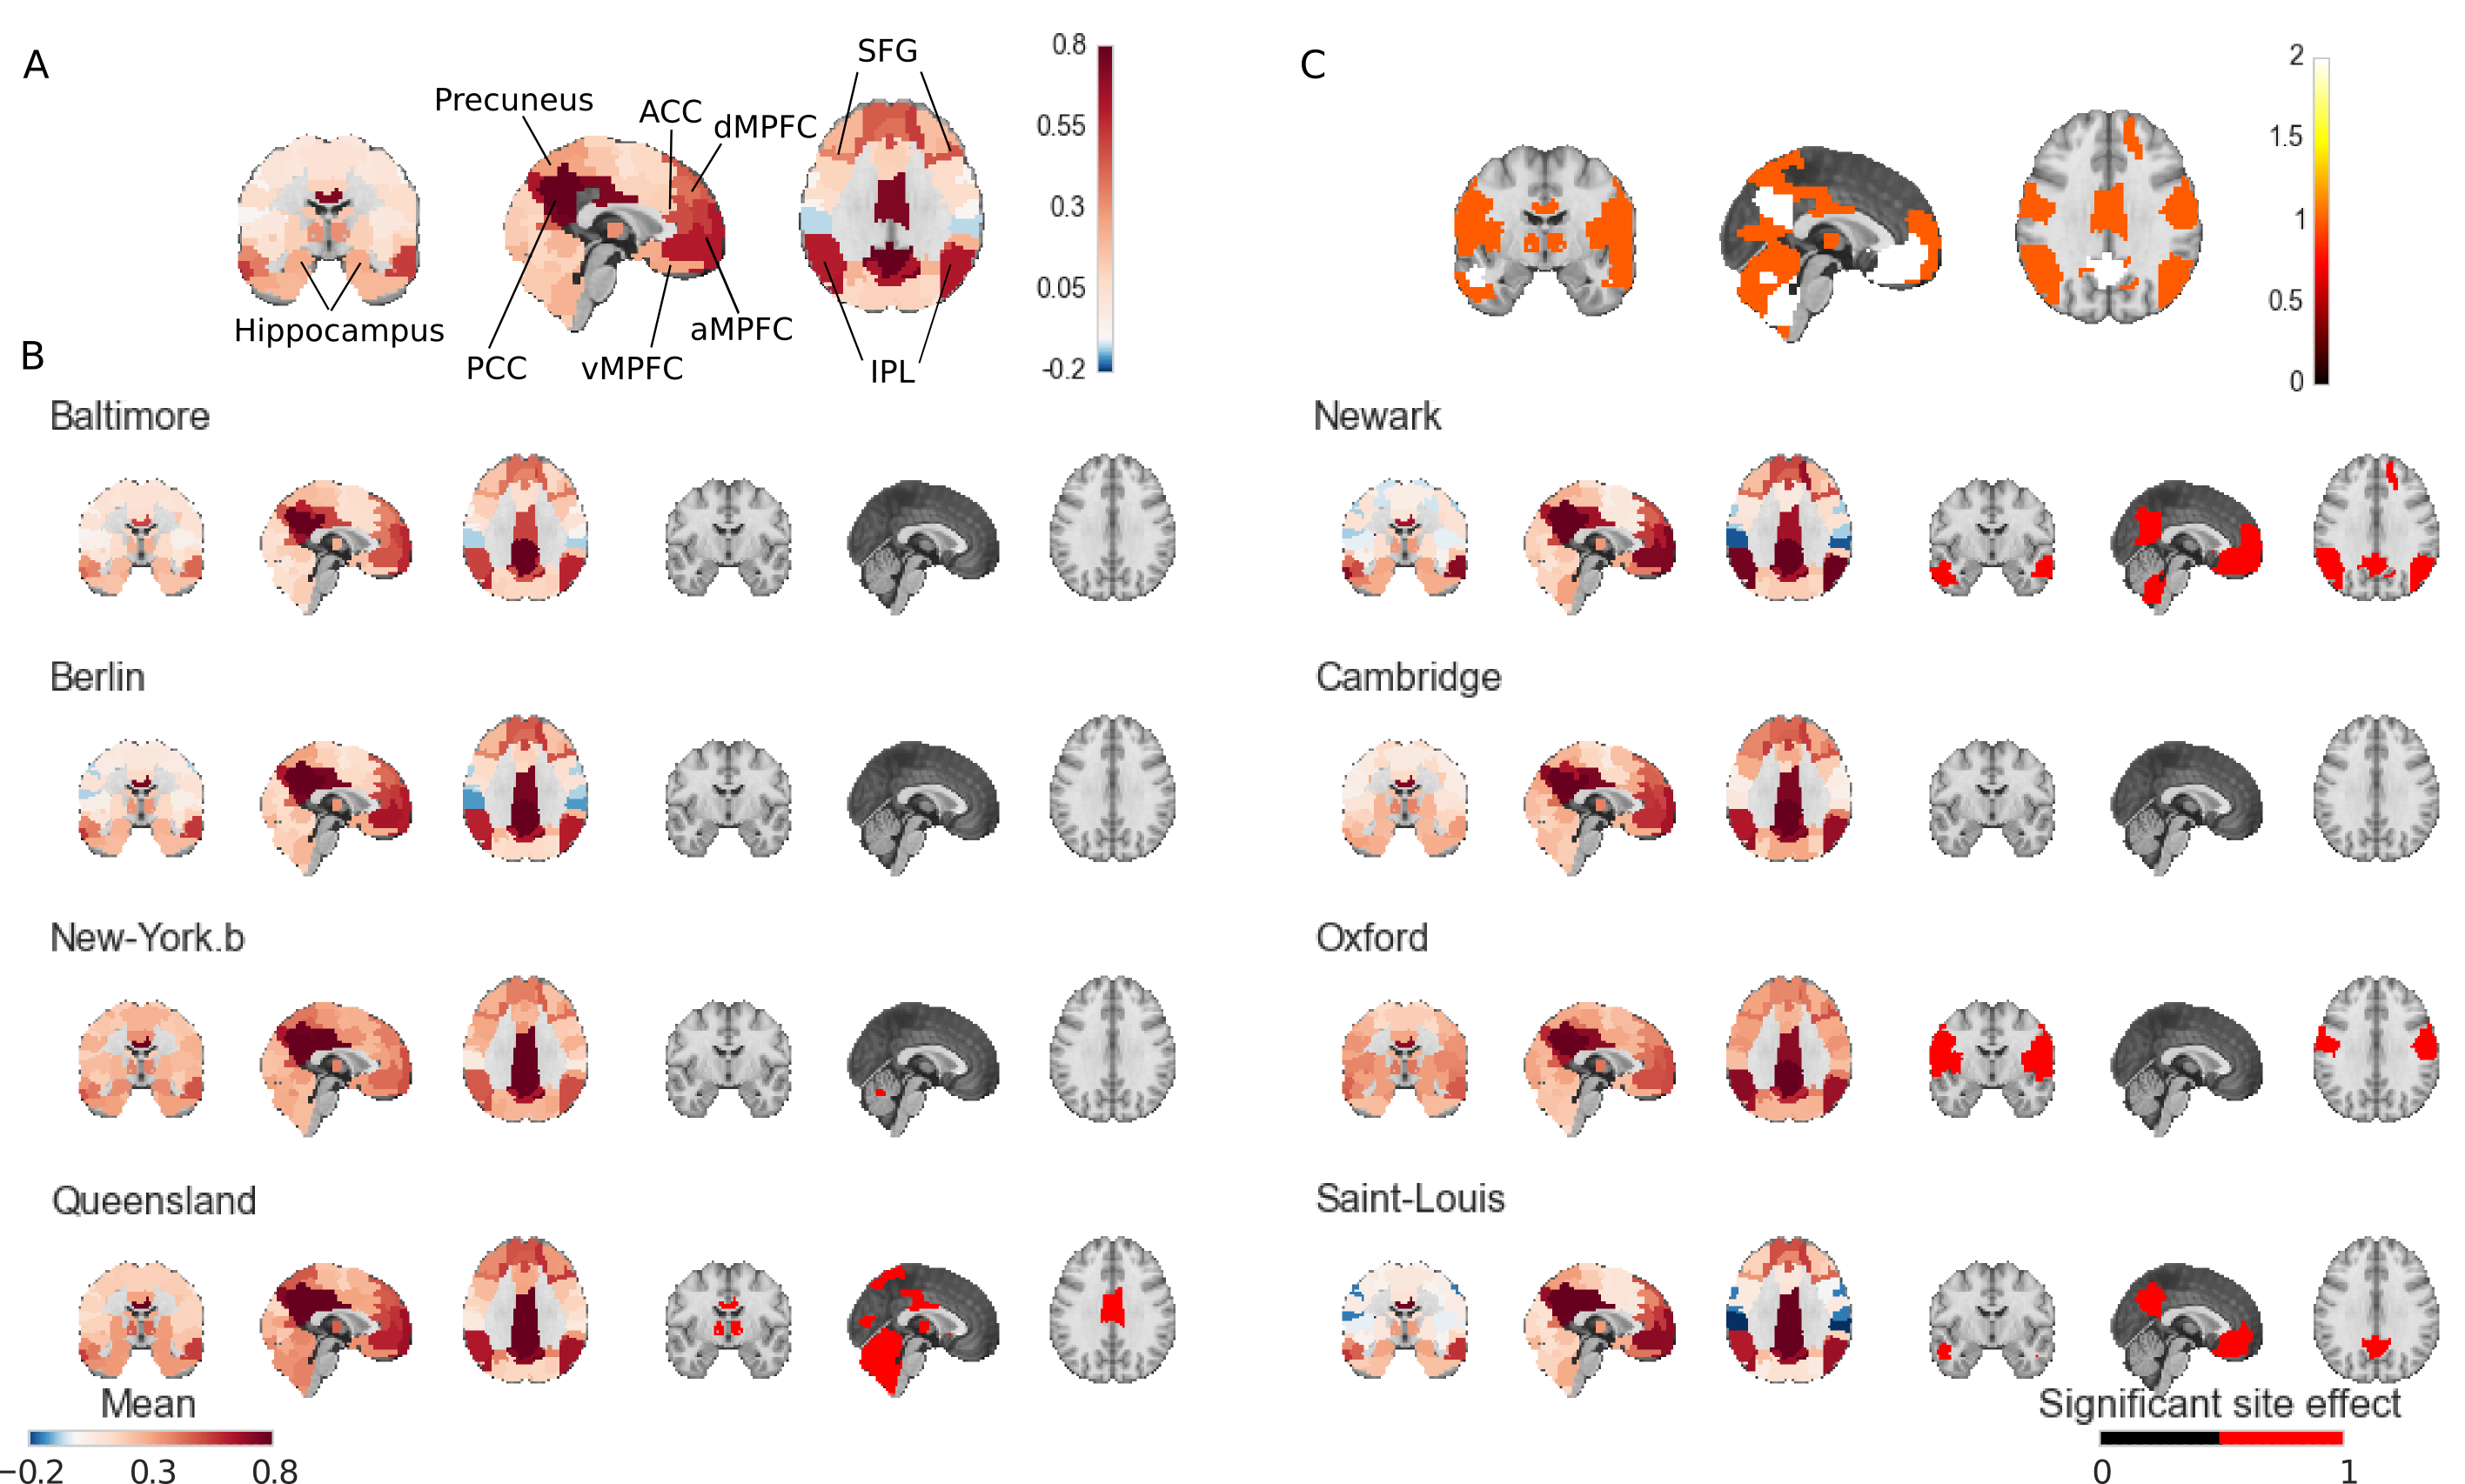
\includegraphics[width=\linewidth]{../figures/dmn_multisite.png}
\end{center}
\caption[DMN variability across sites]{
Panel A: map of the DMN obtained using a seed in the posterior cingulate cortex (PCC), averaging all subjects and sites together. Panels B,C:  The first column show the average functional connectivity maps of the DMN at 8 sites. The second column show the significant differences between the average functional connectivity maps of one site versus all the others. Panel D shows the number of sites with a significant inter-site difference for each brain region.
}
\label{fig_DMN_variability}
\end{figure}

\paragraph{Site bias in the default-mode network} We first focused on the connections associated with a seed region located in the precuneus (PCC), a key node of the default-mode network (DMN) and one of the most widely studied resting-state network \citep{Greicius2004}. The connections were based on the Cambridge $100$ parcellation, and were represented as a connectivity map, Figure \ref{fig_DMN_variability}. Panel Figure \ref{fig_DMN_variability}A shows the PCC connectivity map, averaged across all subjects and all sites. The key regions of the DMN are easily identifiable, and include the PCC, precuneus, inferior parietal lobule, anterior cingulate cortex, medial pre-frontal cortex (dorsal, anterior and ventral), superior frontal gyri and the medial temporal lobe \citep{Damoiseaux2006,Dansereau2014,Yan2013a}. Using a GLM, the average connectivity map of the DMN was then extracted for each site, Figure \ref{fig_DMN_variability}B,C. Qualitatively, the DMN maps were consistent across sites, as expected based on the literature. We then tested for the significance of the site bias, i.e. the difference in average connectivity at a given site and the average connectivity at all remaining sites. The statistical maps were corrected for multiple comparisons across the brain using false-discovery rate (FDR) at $q\leq 0.05$ \citep{Benjamini1995}. A significant bias for at least one connection could be identified for every site, without exception, Figure \ref{fig_DMN_variability}B,C. Figure \ref{fig_DMN_variability}D shows how reproducible were the significant bias in connectivity across the brain and sites. The identified connections were quite variable, most of them identified at less than three sites.

\begin{figure}[htbp]
\begin{center}
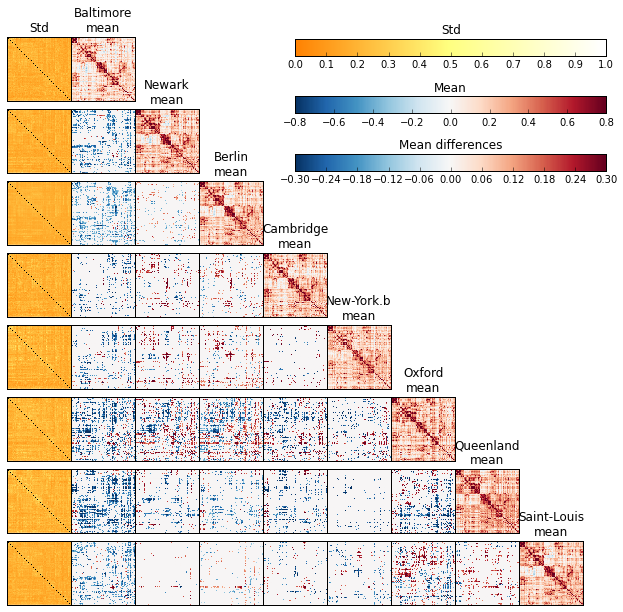
\includegraphics[width=\linewidth]{../figures/connectome_multisite.png}
\end{center}
\caption[Connectome variability across sites]{
Panel A shows the average functional connectomes for 8 sites of the 1000 FCP. Colors next to the $x$ and $y$ axis correspond to different networks in a 7-cluster solution of the matrix, obtained from a hierarchical clustering (Ward criterion). Panel B presents the corresponding 7 brain networks, along with labels. Panel C shows average connectomes for individual sites, as well as connections with a significant site bias. Panel D shows the number of sites at which a given connection was detected as significantly biased. 
}
\label{fig_connectome_variability}
\end{figure}


\paragraph{Site bias across the connectome} In order to extend these observations outside of the DMN, we derived the entire connectome using the Cambridge 100 parcellations. Figure \ref{fig_connectome_variability}A shows the average connectome, pooling all subjects and sites together. The regions have been re-ordered based on a hierarchical clustering (with Ward criterion). A network structure is clearly visible as squares of high connectivity on the diagonal of the connectome (as outlined by black lines). Each diagonal square corresponds to the intra-network connectivity for a partition into 7 networks presented in Figure \ref{fig_connectome_variability}D. These 7 networks were consistent with the major resting-state networks reported using cluster analysis in previous work \citep[e.g.][]{Heuvel2008, Bellec2010, Yeo2011, Power2011}. Specifically, the DMN, visual, sensorimotor, dorsal and ventral attentional networks (dATT and vATT, respectively). A mesolimbic network and cerebellar/visual network were also identified. Figure \ref{fig_connectome_variability}C shows how this large-scale connectome organization varied from site to site. The average connectivity per site as well as significant differences with the average of the remaining sites ($q\leq 0.05$) is presented in Figure \ref{fig_connectome_variability}C. Visually, consistent with our previous observations in the DMN, the organization of the average connectome into large-scale resting-state networks was preserved across all sites. Some significant site-effects were still detected in the connectivity both within each network, as well as in the off-diagonal rectangles highlighting between-network connectivity. By counting the frequency of site showing a significant effect across sites, it was apparent that significant site-effects were quite variable in their localization and spread across the full connectome. 
% The connectome standard deviation across subjects for each site is shown in supplementary material (see \ref{fig_std_connectomes}).

\begin{figure}[htbp]
\begin{center}
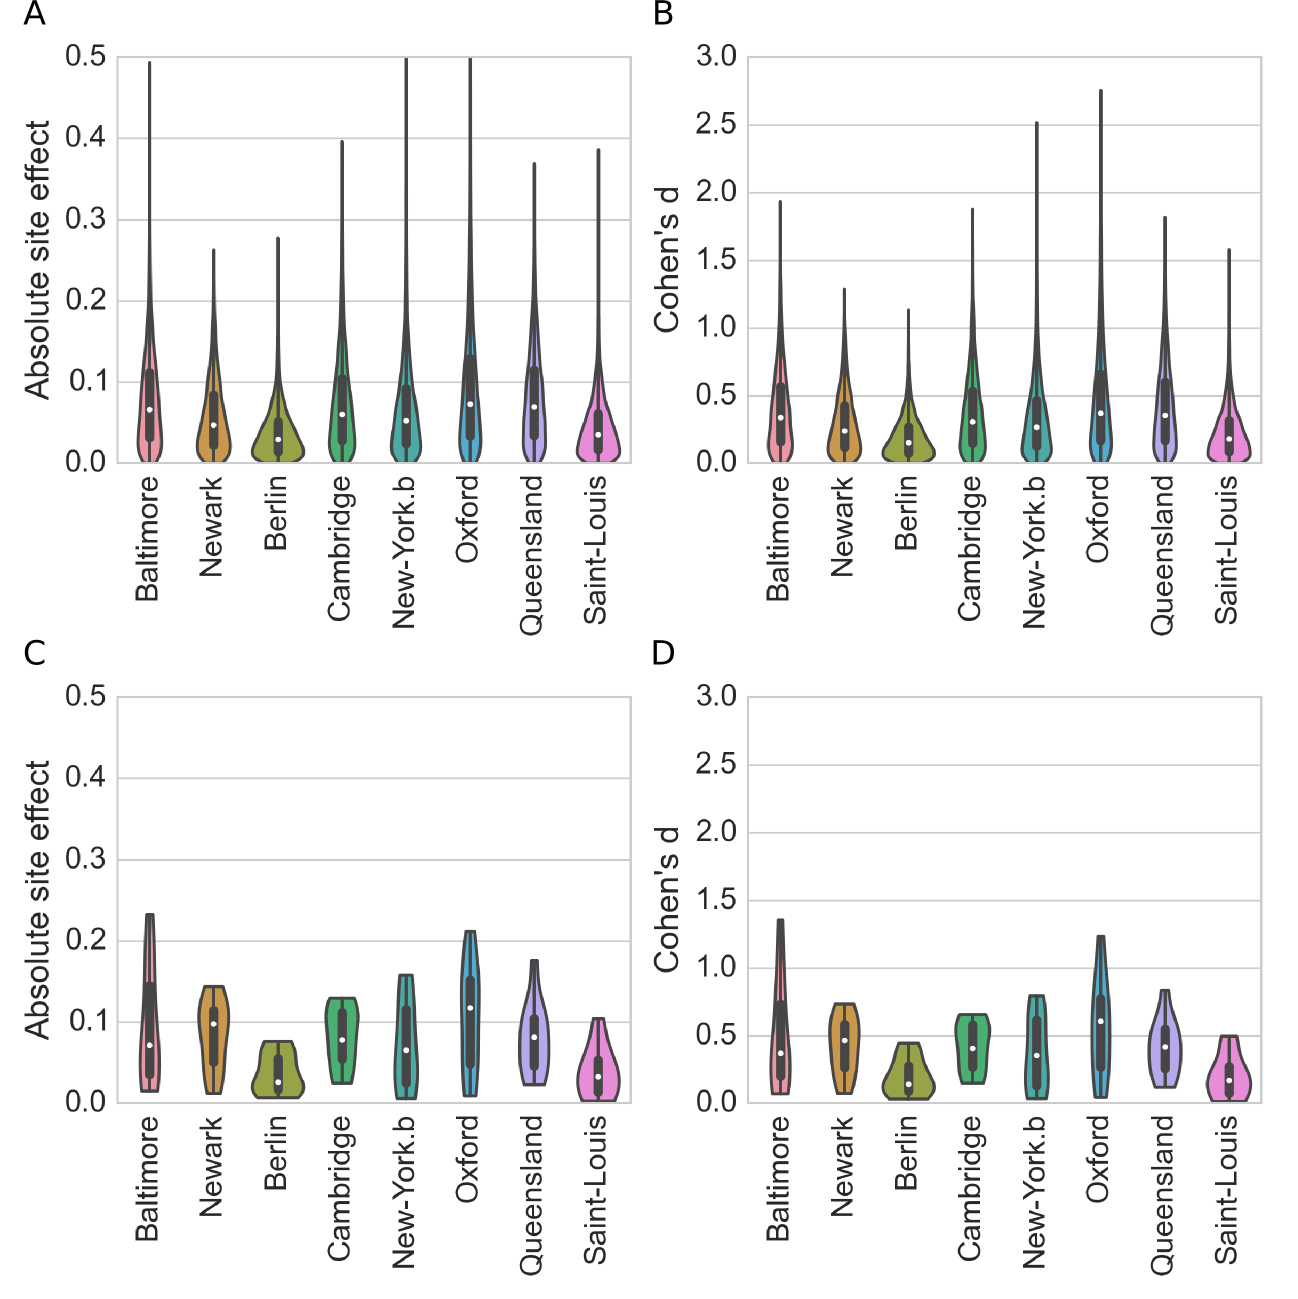
\includegraphics[width=0.8\linewidth]{../figures/effect_distribution.png}
\end{center}
\caption[inter site variability]{
Effect size of the inter-site bias from a subset of 8 sites from the 1000 FCP. Panel A shows the distribution of absolute difference in functional connectivity across all brain connections and Panel C across the selected 11 functional connections. Panel B shows the distribution of of inter-site bias for each connection, expressed as Cohen's $d$ and Panel D across the selected 11 functional connections.
}
\label{fig_site_variability}
\end{figure}
%Distribution of intra-site (between-subject) standard deviation vs. inter-site (between-site) standard deviation, from a subset of 8 sites from the 1000 functional connectome dataset. A) Intra-site standard deviation for each site. B) Inter-site effect size expressed in Cohen's $d$ for eahc site.




\paragraph{Site bias vs within-site variations across subjects} In order to assess how large was the amplitude of inter-site bias in resting-state connectivity measures, we compared it with the variations across subjects within one site, i.e. a Cohen's $d$. Figure \ref{fig_site_variability}A presents violin plots of the (absolute) inter-site bias across all subjects and pairs of connections from the Cambridge parcellation. Figure \ref{fig_site_variability}C restricts the violin plots to the 11 connections selected for Monte-Carlo simulations. The distributions were mostly consistent across sites, with a median around 0.06, $5\%$ percentile near 0 and $95\%$ percentiles in the 0.08-0.1 range. The region-to-region maps of within-site, across-subjects standard deviations are presented for the DMN in Supplementary Figure \ref{fig_std_DMNs}, and for the entire connectome in the Supplementary Material \ref{fig_std_connectomes}. Figure \ref{fig_site_variability}B presents a violin plot of the inter-site bias across all subjects and connections, expressed as Cohen's $d$. In order to compute the Cohen's $d$ values we used the standard deviation from the noise as the reference that was calculated as follow: $std_{error}=\sqrt{\sum{e^{2}}/(N-K)}$ (e being the residual from the GLM, N the sample size and K to the number of covariates in the model) and the Cohen's $d$ was defined as: $|effect|/std_{error}$. Again, the distributions were mostly consistent across sites, with a median around 0.33, $5\%$ percentile near 0 and $95\%$ percentiles in the 0.4-0.6 range. The same findings were found only looking at the 11 pairs of connections that were used in this study shown in Figure \ref{fig_site_variability}D. The effect size of the inter-site connectivity bias was of the order of 0.3 Cohen's $d$. This effect size would be deemed small-to-moderate, which suggests that the impact of additive inter-site bias on statistical tests will be limited. We then proceeded to formally test this hypothesis using Monte-Carlo simulations.

\subsection{Multisite Monte-Carlo simulations}

\begin{figure}[tbp]
\centering
\captionsetup[subfloat]{labelformat=empty}
{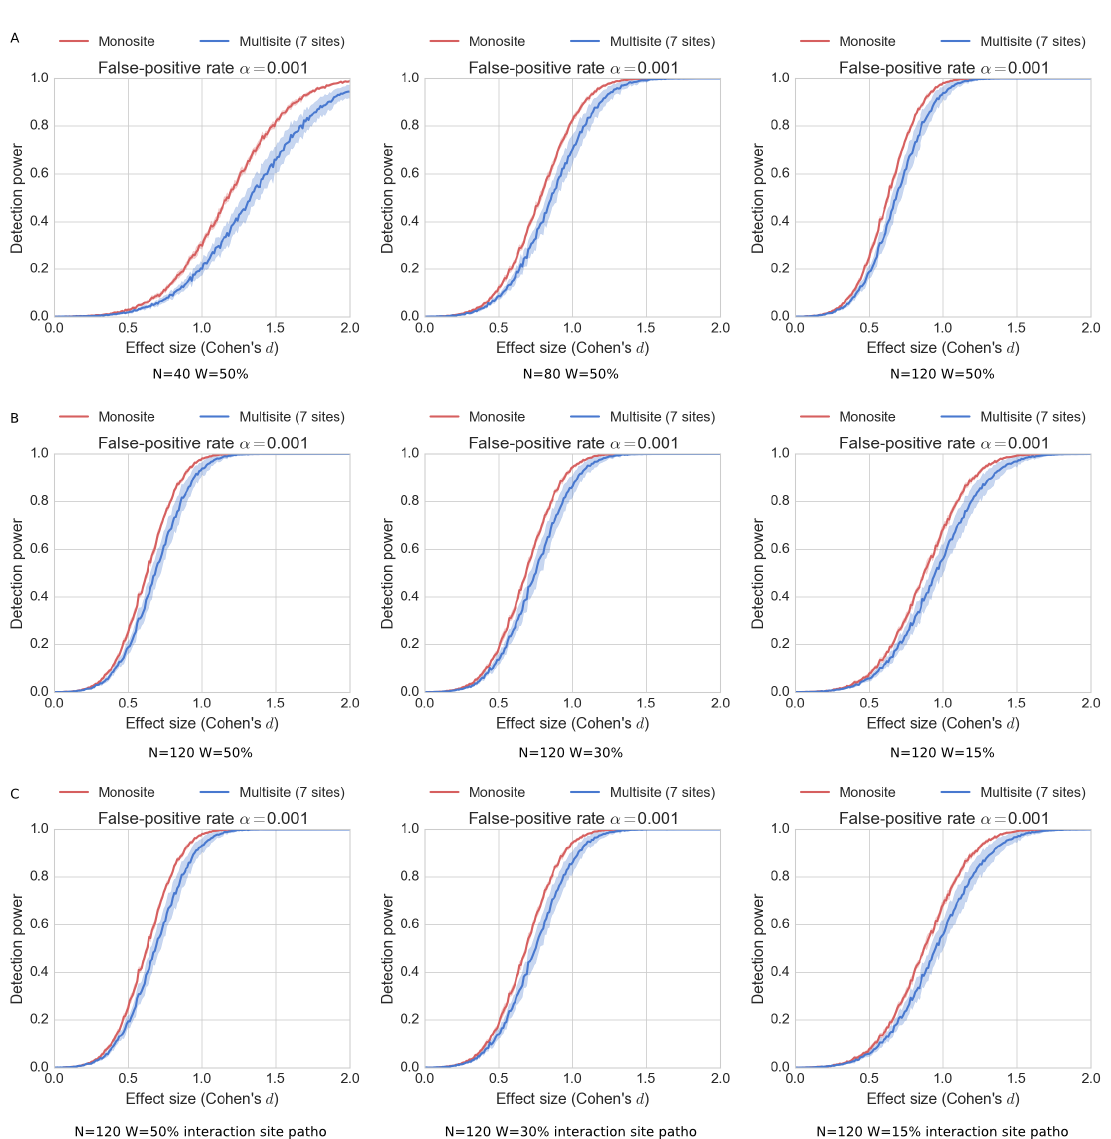
\includegraphics[width=\textwidth]{../figures/simulations_real_7sites.png}}

\caption{
Monte-Carlo simulation of detection power as a function of the effect size $d\in[0,2]$, either for a monosite ($S=1$) or a multisite ($S=7$) sample, when testing differences between two groups with a GLM with a false-positive rate $\alpha=0.001$. In panel A, the patient allocation ratio is fixed ($W=50\%$) and three different sample sizes have been tested, $N\in\{40, 80, 120\}$ (Experiment $(\mathcal{E}_1)$). In panel B, the sample size is fixed ($N=120$) and three different patient allocation ratio have been tested $W\in \{15\%, 30\%,50\%\}$ (Experiment $(\mathcal{E}_2)$).
}
\label{fig_real_sim}
\end{figure}

\paragraph{Statistical power and effect size} Figure \ref{fig_real_sim}A shows the relationship between effect size and a GLM detection power in experiment $(\mathcal{E}_1)$, i.e. for a fixed allocation ratio ($W=50\%$) and three different sample sizes, $N\in\{40, 80, 120\}$. The average and std of detection power was plotted across the 11 selected connections. As expected, the sensitivity increased with sample size, quite markedly. In multisite simulations ($S=7$), for a large effect size ($d=1$), the detection power was $20\%$ with 40 subjects , $80\%$ with 80 subjects and $95\%$ with $120\%$ subjects. The sensitivity was larger with a single site than multisite sample, yet the difference between the two decreased when the sample-size increased. With $N=40$ and $d=1$, the detection power was close to $30\%$ for a single site sampe, compared to $20\%$ for the multisite sample. With $N=120$ and $d=1$, the difference in sensitivity was only a few percents. The same trend was apparent for all tested effect sizes, and also $\alpha\in\{0.01,0.05\}$ (not shown). 
\par
\begin{figure}[htbp]\centering
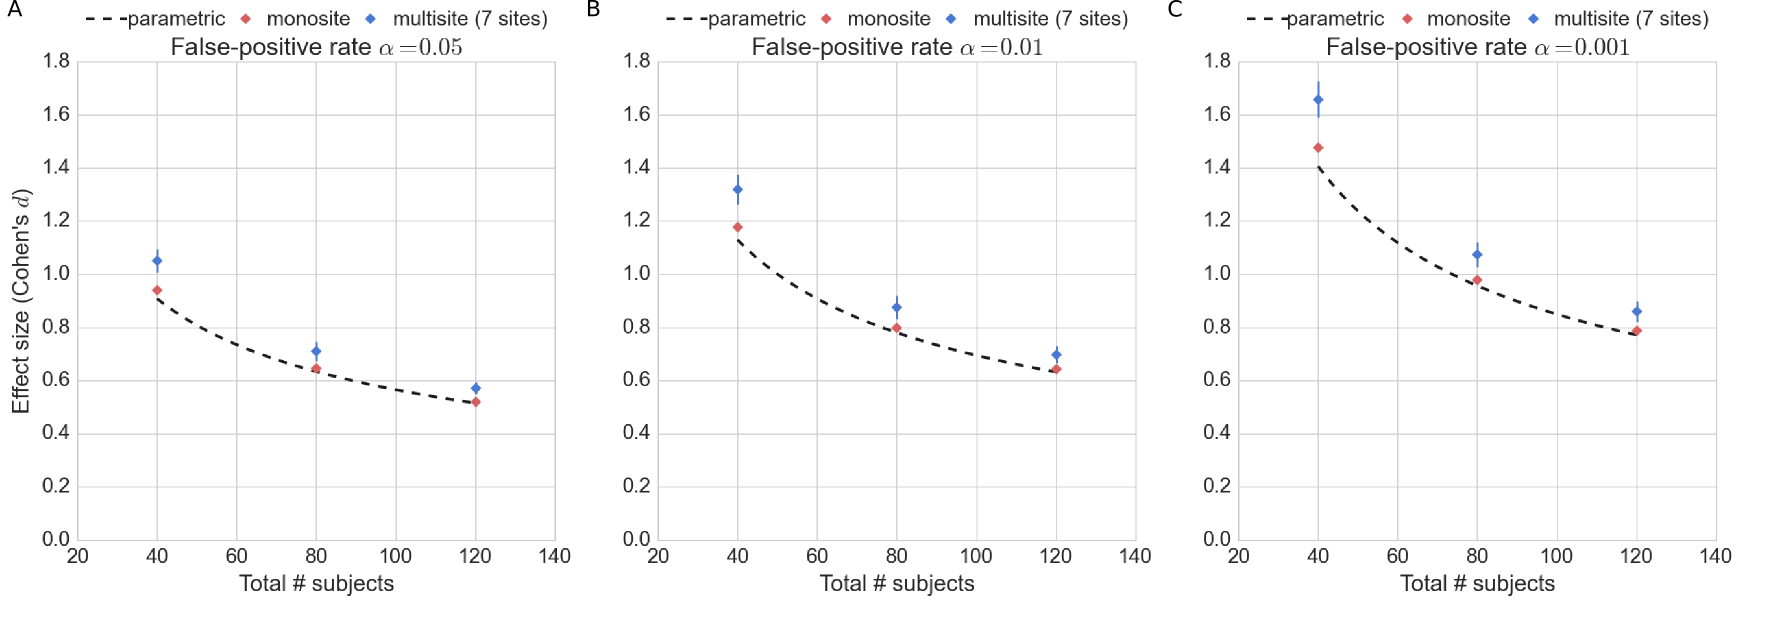
\includegraphics[width=\textwidth]{../figures/samplesize_x_effectsize.png}
\caption[]{
Effect size detectable at 80\% sensitivity as a function of sample size, for different false-positive rate $\alpha\in \{0.05,0.01,0.001\}$ (experiment $(\mathcal{E}_1)$). All simulations used a balanced patient allocation ratio $W=50\%$. The monosite performance is in red and the multisite in blue. The dotted black line shows the detectable effect size for a classical parametric $t$-test. 
}
\label{fig_sampeffect_curves_alpha001}
\end{figure}

\paragraph{Statistical power and group allocation ratio} Figure \ref{fig_real_sim}B shows the relationship between effect size and a GLM detection power in experiment $(\mathcal{E}_2)$, i.e. for a fixed sample size ($N=120\%$) and three different patient allocation ratio, $W\in \{15\%, 30\%,50\%\}$. Overall, we found that the detection power increased with $W$. For example, with $d=1$, the detection power was $65\%$ for $W=15\%$, and increased to $90\%$ with $W=30\%$, and finally $95\%$ for $W=50\%$. The impact of $W$ was observed in both monosite and multisite samples, with an optimal allocation ratio of $W=50\%$ for both. This observation was also made for $\alpha\in\{0.01,0.05\}$ (not shown). 

\paragraph{Detectable effect size, as a function of sample size} An alternative summary of experiment $(\mathcal{E}_1)$ is to represent the effect size that can be detected with 80\% sensitivity, as a function of sample size for monosite and multisite configurations, see Figure \ref{fig_sampeffect_curves_alpha001}. As a reference, we computed the same curve for parametric $t$-test comparisons, under assumptions of normality. As exepcted, the detectable effect size for parametric $t$-tests closely followed the monosite estimation, with the notable expection of small sample sizes ($N-=40$. For small sample size ($N=40$), the detectable effect size was notably larger in multisite configuration than in monosite configuration (difference of about 0.25 in Cohen's $d$ for $\alpha=0.001$. However, the difference decreased for large sample size to become smaller than 0.1 with $N=120$ and $\alpha=0.001$. The lowest detectable effect size for a sensitivity of $80\%$ at $\alpha=0.05$ is about $d=0.8$, achieved in monosite configuration with $N=120$. At this sample size, the difference between single and multisite configurations was marginal, with only a few percent of difference in detectable effect sizes. 


\begin{figure}[tbp]
\centering
\captionsetup[subfloat]{labelformat=empty}
{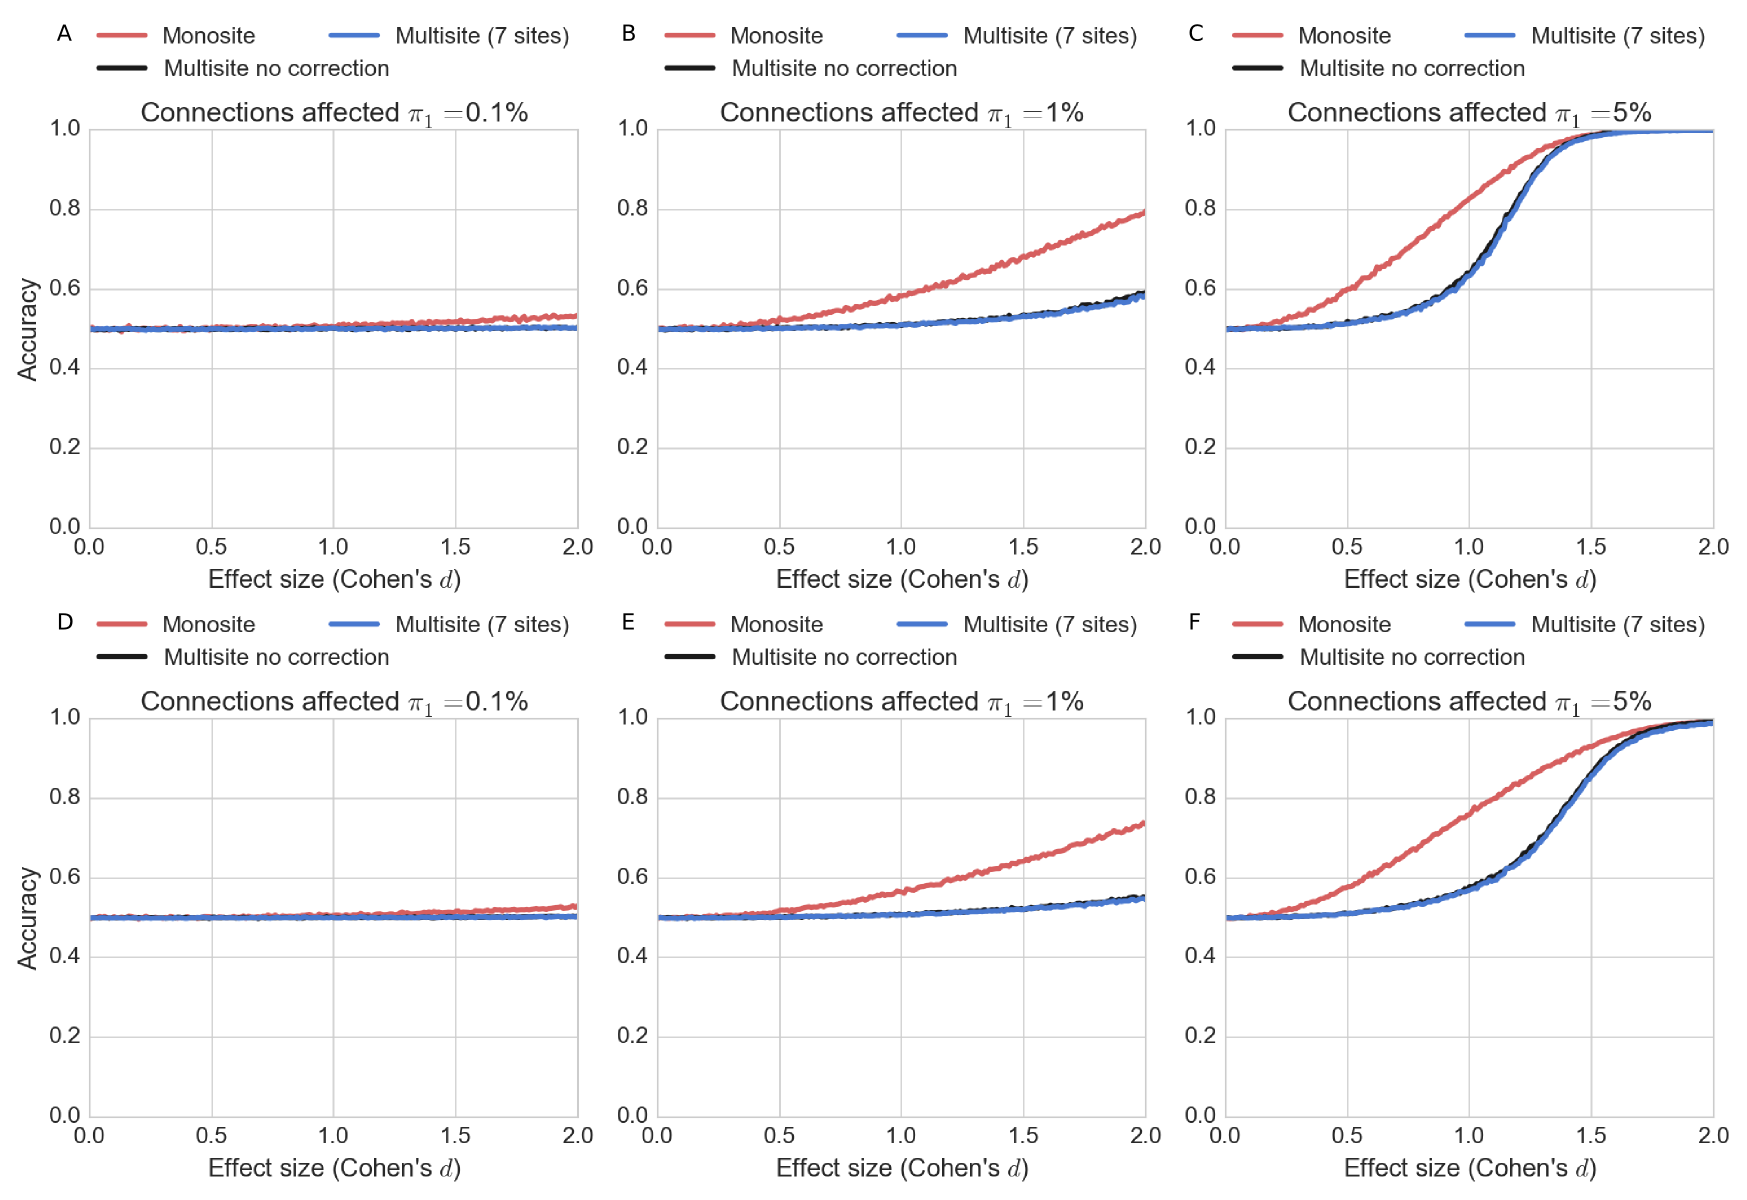
\includegraphics[width=\textwidth]{../figures/prediction_effectsize.png}}
\caption{
bala
% Prediction accuracy of patient vs controls as a function of effect size. Three simulation settings are presented on each plot: monosite (red curve), multisite with regression of site effects ($S=7$, blue curve), and multisite without regression of site effects ($S=7$, black curve). Accuracy was estimated over $B=1000$ simulation samples with a patient allocation ratio $W=50\%$ and 3 volumes of affected connections $\pi_1\=0.1\%$ (left column), $\pi_1\=1\%$ (middle column) and $\pi_1\=5\%$ (right column). Two sample sizes were tested: $N=120$ for training, with $N=28$ to estimate accuracy (first row), and randomly selected subjects and model accuracy was estimated on the remaining $28$ subjects. For Panel D,E,F the training of the SVM model is performed on
% $N=80$ for training, with $N=68$ to estimate accuracy (second row). 
}
\label{fig_prediction_sampeffect}
\end{figure}


\paragraph{Prediction accuracy}
In experiment $(\mathcal{E}_3)$, we examined the impact of effect size and the volume of affected connections on prediction accuracy in a SVM, see Figure \ref{fig_prediction_sampeffect}. The volume of changes $\pi_1$ had a major impact prediction accuracy. At $\pi_1=0.1\%$ (around 5 connections) the accuracy level was at chance level across all tested effect sizes, Figure \ref{fig_prediction_sampeffect}A. With $\pi_1=1\%$, Figure \ref{fig_prediction_sampeffect}B, accuracy slightly increased, but effect sizes larger than $d=2$ were still required to reach over $80\%$ accuracy. With $\pi_1=5\%$, $95\%$ accuracy was achieved at the same effect size (about $d=1.5$) for monosite and multisite simulations, although the accuracy in multisite simulations was notably lower than for monosite simulations across most effect sizes, see Figure \ref{fig_prediction_sampeffect}C. The relatioship between effect size and accuracy followed a sigmoidal curve in both settings, yet a sharper, and latter transition between very low and very accuracy was observed in multisite simulations. Interestingly, correcting for site effects by regressing out the dummy variable before running the SVM classifier had no impact on accuracy levels. The sample size ($N=80$ vs $N=120$ for training) did have a moderate effect on prediction accuracy: for $\pi_1=5\%$ and $d=1$ and monosite simulations, accuracy was about 85\% with $N=120$ (Figure \ref{fig_prediction_sampeffect}C) and 75\% with $N=80$ (Figure \ref{fig_prediction_sampeffect}F). \emph{Please add $N$ in the figures, next to ``accuracy'' on the y axis, not just the legend}.

%%%%%%%%%%%%%%%%%%%%%%%%%%%%%%%%%%%%%%%%%%%%%
% END of results section                    %
%%%%%%%%%%%%%%%%%%%%%%%%%%%%%%%%%%%%%%%%%%%%%

\section{Conclusions and discussion}

% What is a reasonable alpha value?

\paragraph{Inter-site bias in rs-fMRI connectivity} Typical resting-state networks were reliably found across sites, such as the DMN, the vATT, dATT, Visual and SM networks. This was strongly expected given the relative consistency of their distribution across individuals, studies, preprocessing approaches or even methods used to extract networks \citep{Damoiseaux2006,vandeheuvel2008,Bellec2010c,Yeo2011,Power2011}. We however found that significant differences in average connectivity (bias) existed between the sites, as previously reported by \citep{Yan2013a}. This connectivity bias may undermine the generalization of the results derived at a single site. The inter-subject (intra-site) standard deviation of the connections was found to be 2 fold greater than the inter-site absolute bias. This effect size measured in Cohen's d would be deemed small-to-moderate, which suggests that the impact of additive inter-site bias on statistical tests will be limited. A reassuring finding in favour of the feasibility of statistical tests pooling fMRI data across multiple sites.\\

%\paragraph{Spatial distribution of connectivity bias} We found that the brain connections exhibiting significant inter-site bias were quite variable, with most of them identified in less than one fourth of the sites. This suggests that there are no large network-specific inter-site bias or that the statistical power for detecting bias with the employed site sample-size was limited. Looking at the spatial location of the site bias with respect to a partition in 7 networks, we noticed that the DMN and the dATT networks were less affected by site bias then the cerebellar, mesolimbic and sensory-motor networks \emph{did we really observe that? CD: Yes looking at the matrix of figure2D I could observe a bit more difference from one network to the other I can compute the average of the value in each network that would give use a cleaner picture... }. This last finding may be associated with the fact that those network are more on the periphery of the brain and may be more sensitive to motion artifacts. 

\paragraph{Statistical power and multisite rs-fMRI} The multisite simulation polling 7 sites showed, after accounting for site-related differences (explicit correction for multi-site variability using dummy variables), similar detection power although slightly lower for the multisite configuration. However, the difference between a monosite and a multisite study was smaller as we increase the sample-size. Another compelling proof of the lack of statistical power at small sample-sizes is the study reported by \cite{Nielsen2013} where they did an analysis on a single site dataset and a multi-site dataset of subject with autism and concluded that the multi-site autism study classification accuracy significantly outperformed chance but was much lower for multi-site prediction than for previous single site results. We therefore need to keep in mind that the site-effect must be taken in account in the analysis and that we may suffer a small lost in detection power for a given effect size in a multisite configuration compared to an equal size monosite study.\\
\par
Second for a given detection power the lowest effect size that we are able to detect is more variable across connections for a low sample-size and decrease as we increase the sample-size.  
An observation promoting the use of large sample-size ($>100$ subjects) for multisite studies. Note that this is probably greatly influence by the number of sites that one will pool to achieve a final given sample-size. 

%Second the Cohens's $d$ achieve for a given sample-size is also a lot more variable among connections with low sample-size compared to larger sample-size \emph{This sentence is crytpic. Beyond the form, what may cause that?}. \emph{Resulting in the following conclusion combining large site may results in low bias compared to very small sites. It is therefore better to have a few large sites then a large number of small sites.I am pretty sure we did not test that. We had 7 small vs 7 large sites. We did not compare a few sites vs many sites with the same sample-size}. 

%\par
%\emph{At this stage, you are done discussing your findings in direct relationship with your objectives. Now is time to discuss limitations, implications and also potential avenues of future work}. 

\paragraph{Statistical power and sample-size} For an effect size considered as medium, e.g. 0.5, the sensitivity was low (below $20\%$), even for monosite simulations with $120$ subjects (Figure \ref{fig_real_sim}A). This is a sobering reminder that with the low false-positive rate typically used in rs-fMRI studies, resulting from correction for multiple comparisons, the sensitivity is quite limited even for over 100 subjects. In particular, our results suggest that resting-state studies based on 40 subjects or less, even at a single site, may be seriously under-powered, unless the effect under investigation were extremely large (Cohen's $d$ greater than 1.5). Also in both cases (monosite and multisite) the effect of unbalancing the two populations may greatly reduce our capacity to detect changes e.g. for an effect size of 1 the detection power goes from $95\%$ in a balanced case to $65\%$ for an unbalanced dataset (allocation ratio $W=15\%$). We therefore recommend to favour balanced dataset when pooling them in order to reduce the variance.

\paragraph{Prediction}
Comparing the monosite and the multisite accuracy curves we have a substantial drop of accuracy from monosite to multisite but this will be to the benefit of generalization, which is an acceptable drawback. Another interesting point is that to achieve a $95\%$ accuracy both monosite and multisite need the same effect size. The monosite is more linear in it's relationship to effect size and the multisite in behaving more like a sigmoidal curve reaching the same level of accuracy as the monosite at hight accuracy level.

One of the main and most interesting finding for the prediction simulations is the fact that multivariate analysis seams to require no linear correction for site-effect before training since the accuracy curve of the multisite with and without correction are perfectly overlapping. The model seam to learn to be invariant to the site-effect as long as we provide him with representative examples of that said variance in the training set. As expected the sample-size for the training set greatly improve our sensitivity to smaller effect size, going from an effect size of 1.4 Cohen's $d$ for an accuracy of $80\%$ with $80$ subjects (see Figure \ref{fig_prediction_sampeffect}F) to 1.2 Cohen's $d$ with $120$ subjects (see Figure \ref{fig_prediction_sampeffect}C). Finally the extent of the affected connections seams to be an important variable, suggesting that feature reduction and/or selection is a very important step to improve our sensitivity to small effect sizes.


\paragraph{Underlying causes of the site bias}
Not all sites seemed to be equally biased, with sites like Berlin or Saint-Louis showing a small number of connections significantly different then the grand average connectivity matrix, while sites like Baltimore, Queensland and Oxford showed much more biased connectivity measures. This may simply be a statistical fluke or a reflection of the protocol or scanner characteristics of these sites. Multiple cause may be interacting together to produce the site bias, like reported by \cite{Yan2013a}, although some of these sources of variance could be better controlled like the scanner parameters paired with the use of a phantom to promote more homogeneous configurations across site and a close monitoring of the experimental paradigm across-site as proposed by \cite{Friedman2006,Friedman2006a,Glover2012}. Although even in standardized study with a great effort made on homogenizing the scanners protocol differences remain \cite{Brown2011}. A much larger site sample with varying parameters could enable a data-driven identification of the critical parameters impacting site bias. The various releases made by the INDI initiative may fill that gap in the literature in the future, as the scanner protocols are much better described in recent releases such as CoRR than they were in the initial FCP release. There will however still be a bias that may be related to local recruitment strategies, the characteristics of local population, or undocumented aspects of the study such as training of subjects to the scanning environment. Many physiological factors are likely to be contributing to these variations, such as the cognitive state of the subject, the level of alertness/drowsiness, circadian rhythm, hunger, medical regimen, potential neurostimulants, amongst others. 

Our study show simulation using real data of heterogeneous protocols on 7 scanners compared to the majority of the literature on the subject comparing two sites homogeneous sites \citep{Costafreda2007,Suckling2008,Sutton2008,Glover2012} and three sites for \cite{Gountouna2010}. As opposed to \cite{Sutton2008,Brown2011} who reported a 10 times smaller contribution of the inter-site variance compared to the inter-subject variability, we have observed a 2 times smaller contribution. There is mainly 2 factors that may contribute to an increase in site variance and explain this difference in site variation, namely the number of sites involved in the study and the degree of homogenization of the protocols and experiments. Also a word of caution should be made regarding the fact that the great majority of scanner were Siemens, and therefore more variability may be found using various scanner manufacturer unfortunately this avenue was not testable using this dataset.

\paragraph{Other types of multisite data} Another limitation is in the case of very large number of site with a few subjects per site, which is common for the recruitment of patient populations in a limited time frames, e.g. the Alzheimer’s disease neuroimaging initiative (ADNI) \citep{Mueller2005} and fBIRN \citep{Friedman2006,Friedman2006a}, and in pharmaceutical clinical trials at phase II and III \footnote{\url{http://www.roche-trials.com/trialDetailsGet.action?studyNumber=BP28248}}. An important benefit of multisite acquisitions is to offer improved generalization compared to single site studies, due to more diversity in scanners and populations. In this case the multisite effect may be more pronounce then what we observed with 7 sites, although the detection power between monosite and multisite diminish with the sample-size and may be negligible for samples greater then 200 subjects. Unfortunately this hypotheses could no be tested with the current dataset due to the limited number of sites available. In future work given an appropriate dataset it would be interesting, using a similar approach, to test if the added variability introduce by the use of a large number of sites with a small number of subjects/site will be compensated by the sample-size as hypothesized in this study.

\paragraph{Beyond additive bias} Also the generative model used for our simulations was based on the hypotheses of an additive effects of the pathology and site, therefore the results and conclusions can only be valid if the model investigated is in fact an additive effect model. Other effects types may include but are not limited to interactions of the site and pathology, polynomial and non-linear interaction.

\section{Acknowledgments}
Parts of this work were presented at the 2013 annual meetings of the organization for human brain mapping, as well as the  Alzheimer's Association International Conference (AAIC) (2013) (Boston) \citep{Dansereau2013b}. The authors are grateful to the members of the 1000 functional connectome consortium for publicly releasing there datasets. The computational resources used to perform the data analysis were provided by ComputeCanada\footnote{\url{https://computecanada.org/}} and CLUMEQ\footnote{\url{http://www.clumeq.mcgill.ca/}}, which is funded in part by NSERC (MRS), FQRNT, and McGill University. This project was funded by NSERC grant number RN000028, a salary award from ``Fonds de recherche du Qu\'ebec -- Sant\'e'' to PB as well as a salary award by the Canadian Institute of Health Research to CD.

\section*{References}

\bibliographystyle{elsarticle-harv}
\bibliography{cdansereau}


\pagebreak



\clearpage
\appendix


%% SUPPLEMENTARY MATERIAL
\clearpage
\pagebreak
\renewcommand{\thefigure}{S\arabic{figure}}
\renewcommand{\thetable}{S\arabic{table}}
\setcounter{figure}{0}
\begin{center}
\emph{Supplementary Material {--} Statistical power and measurement bias in multisite resting-state fMRI connectivity}\\

\vspace{\baselineskip}Submitted to Neuroimage.\\

\vspace{\baselineskip}C. Dansereau$^{1,2}$,  Y. Benhajali$^{1}$,C. Risterucci$^{3}$, E. Merlo Pich$^{3}$, P. Orban$^{1}$, D. Arnold$^{4}$, P. Bellec$^{1,2}$\\

\end{center}
$^1$Functional Neuroimaging Unit, Centre de Recherche de l'Institut Universitaire de G\'eriatrie de Montr\'eal\\
$^2$Department of Computer Science and Operations Research, University of Montreal, Montreal, Quebec, Canada\\
$^3$F. Hoffmann-La Roche Ldt., Basel, Switzerland\\
$^4$NeuroRx, Montreal, Quebec, Canada\\

For all questions regarding the paper, please address correspondence to Pierre Bellec, CRIUGM, 4545 Queen Mary, Montreal, QC, H3W 1W5, Canada. Email: pierre.bellec (at) criugm.qc.ca.\\

\section*{Supplementary Material} 

\begin{figure}[tbp]
\centering
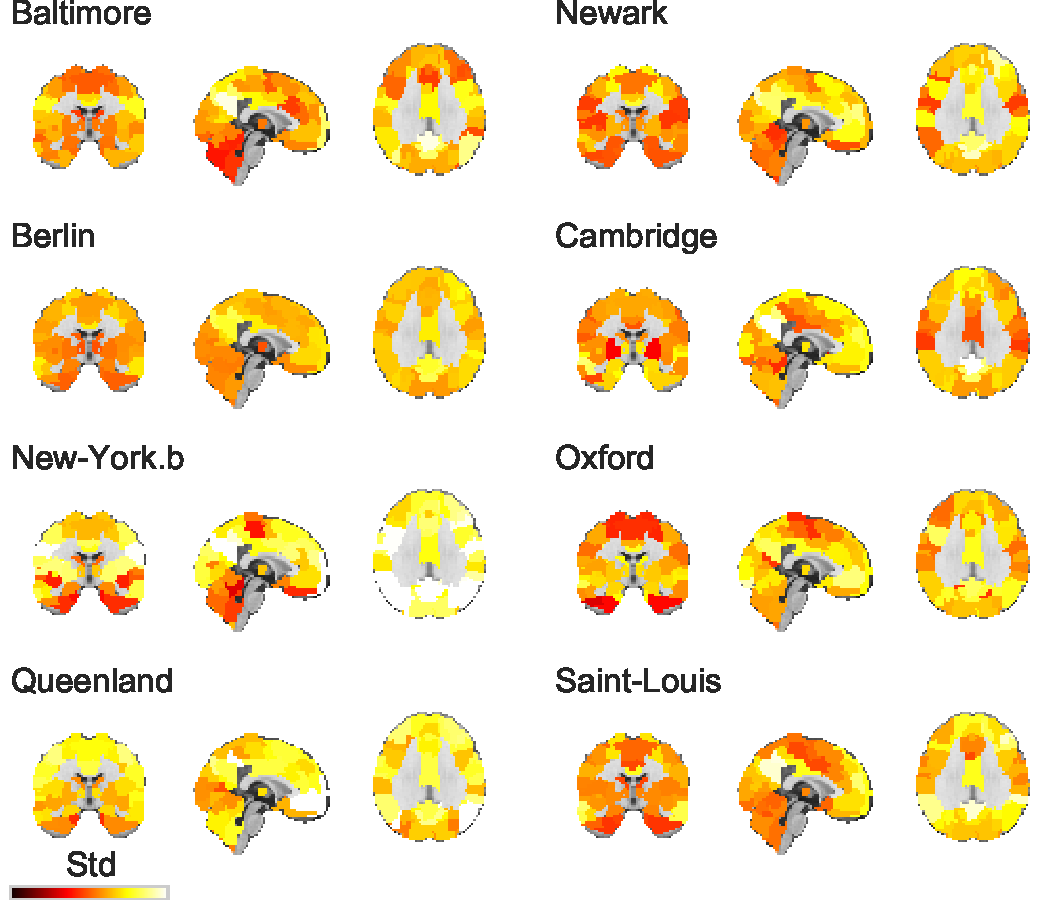
\includegraphics[width=0.75\textwidth]{../figures/dmn_stdmultisite.pdf}
\caption[]{
Overlay of the standard deviation of the DMN for each site on the MNI152 template.
}
\label{fig_std_DMNs}
\end{figure}

\begin{figure}[tbp]
\centering
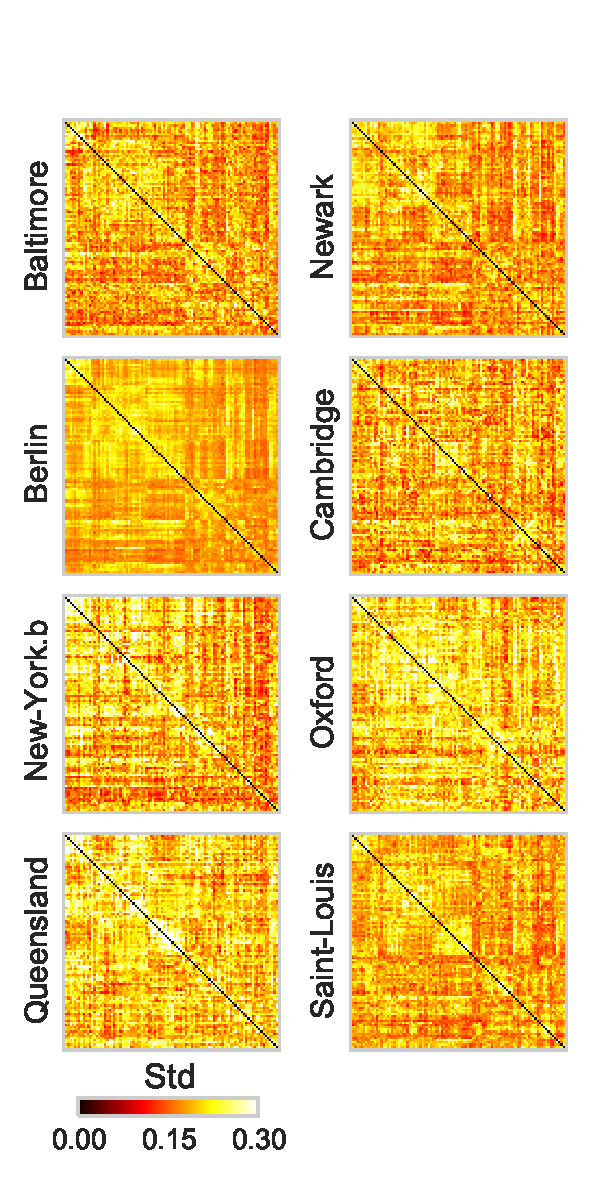
\includegraphics[width=0.50\textwidth]{../figures/connectome_std_multisite2.pdf}
\caption[]{
The standard deviation of the connectome for each site.
}
\label{fig_std_connectomes}
\end{figure}


Figure \ref{fig_real_sim_debalancing_2sites} show a scenario of two sites one large (80 subjects) and one small ($\sim20$ subjects) unbalanced at an allocation ratio $W$ of 30\% and the inverse ($W=$70\%). As we can see the multisite configuration is as good as the monosite and the variance between connection is of the same order for the monosite and multisite.

\begin{figure}[tbp]
\centering
\captionsetup[subfloat]{labelformat=empty}
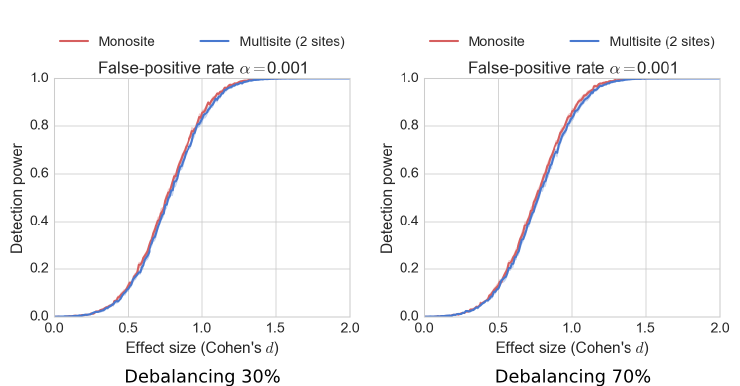
\includegraphics[width=.75\textwidth]{../figures/simulations_real_2sites.png}
\caption{
Simulation on real data, detection power of two groups for a total of 100 subjects between 2 sites, one small site of 20 subjects and one large of 80 subjects. Every plot show two scenarios, 1) monosite and 2) multisite 2 sites with correction for multisite differences using dummy variables. Each plot show the detection power in function of the effect size for 2 different allocation ratio $W$ of 30\% and 70\% between 2 sites.
}
\label{fig_real_sim_debalancing_2sites}
\end{figure}


\end{document}


